%%=============================================================================
%% Eventual Consistency
%%=============================================================================

\section{Eventual Consistency}
\label{sec:eventual-consistency}

Elk commando dat in het systeem terecht komt, kan op een queue geplaatst worden. Het grote voordeel hiervan is dat het systeem niet overbelast wordt en dat elke queue job afgehandeld kan worden \autocite{King2015EventualConsistency}. Vandaar de term eventual consistency, uiteindelijk zal het systeem consistent zijn. Een ander groot voordeel is dat eventual consistency automatisch samen kan werken met schaalbaarheid van een applicatie, zoals beschreven in Hoofdstuk~\ref{ch:schaalbaarheid}. Wanneer er een commando uitgevoerd wordt op het systeem, kent de client reeds de nodige data die hij net verstuurd heeft. Er is momenteel geen nood om meteen een respons terug te krijgen.
Daarom is het ook belangrijk bij commands om een \gls{GUID} op voorhand te definiëren zodat de identiteit al bekend is. Met deze identiteit kan er eventueel al een pagina getoond worden waar de nieuwe data weergegeven wordt.

\begin{figure}[h]
\caption{Eventual Consistency}
\centering
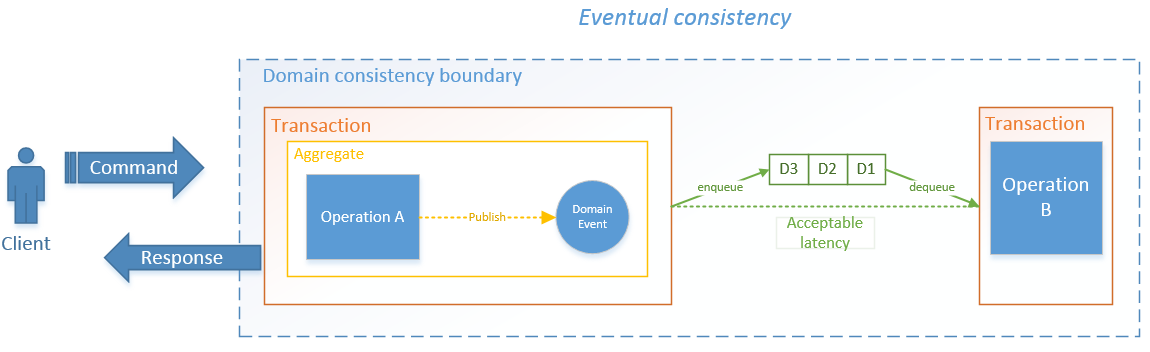
\includegraphics[width=0.75\textwidth]{img/eventual-consistency}
\end{figure}

\subsection{Transactional Consistency}
\label{subsec:transactional-consistency}

Het voordeel aan transactional consistency is dat de respons meteen terug gegeven wordt. Alle delen van de applicatie zijn doorlopen en alle gegevens zijn gepersisteerd. De grote nadelen zijn dat de applicatie volledig doorlopen moet worden of dat de applicatie een exponentieel hoog aantal \glspl{request} binnen krijgt en dus alles meteen moet afhandelen. Hierdoor kan de respons veel trager zijn en dit kan resulteren in het crashen van de applicatie.
Transactional consistency is ook moeilijker schaalbaar omdat alles in 1 keer uitgevoerd wordt.

\begin{figure}[h]
\caption{Transactional Consistency}
\centering
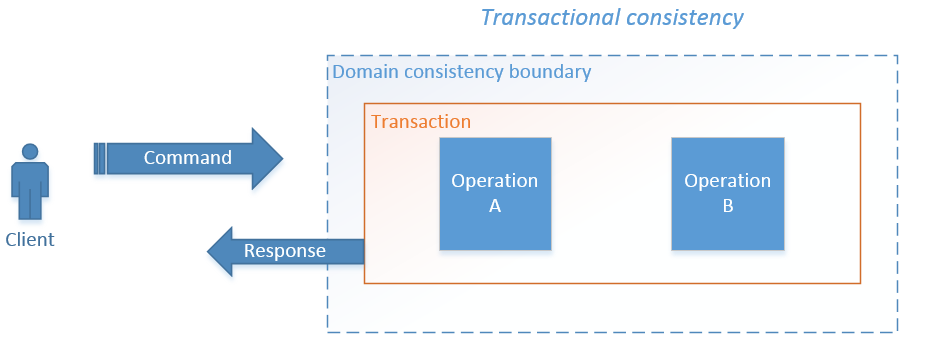
\includegraphics[width=0.75\textwidth]{img/transactional-consistency}
\end{figure}
